\chapter{GPGPU - Obecné výpočty na grafické kartě}  \label{sec:gpgpu}
Obecné výpočty na grafické kartě (anglicky General-Purpose computing on graphics processing unit, zkratka GPGPU) využívají výpočetní síly grafických procesorů, které byly původně navrženy pouze pro výpočty v počítačové grafice. Ve spolupráci s CPU jsou ale v tomto případě využívány k řešení obecných úloh, které jsou normálně zpracovávány pouze CPU.\\

Protože řešení grafických úloh vyžaduje většinou mnoho vektorových a maticových výpočtů, které jsou mnohdy snadno paralelizovatelné, obsahuje architektura GPU mnoho jednoduchých výpočetních jader schopných počítat základní matematické operace a pracovat paralelně. Jejich hlavní výhodou oproti běžným CPU, je tady fakt, že obsahují stokrát, v poslední době až tisíckrát, více jader navržených k paralelním výpočtům, takže pokud je úloha dobře paralelizovatelná a vyžaduje pouze jednoduché matematické úlohy, můžeme její výpočet urychlit až tisícinásobně v porovnání s CPU.\\

Z počátku podporovaly grafické karty pouze vektorové a maticové výpočty s dimenzí 2, 3 nebo 4, protože se tyto struktury běžně používají v grafických výpočtech. Pokud jsme tedy chtěli počítat běžné úlohy, bylo potřeba je přeformulovat a složit pouze z grafických operací podporovaných grafickými rozhraními jako je DirectX či OpenGL. Tato transformace byla pro programátory velmi náročná a často dokonce nemožná, takže mnoho algoritmů nemohlo výpočetní potenciál grafických karet využít.\\

Tento problém ale zmizel s příchodem specializovaných nástrojů pro využití GPU pro obecné výpočty. Tyto frameworky umožňují vývojářům oprostit se od limitací daných grafickým prostředím a využít GPU k obecným výpočtům mnohem jednodušeji.~\cite{Kirk12}\\

V dnešní době existují 2 hlavní frameworky pro GPGPU, konkrétně CUDA~\cite{Sanders10} a OpenCL~\cite{Scarpino11} (open computing language). CUDA má oproti konkurenčnímu OpenCL velkou výhodu v přímé vazbě na hardware. Je to dáno tím, že CUDA je vyvíjena firmou Nvidia pouze pro vlastní karty, takže může využívat specifických vlastností konkrétní architektury. V porovnání s tím je OpenCL od skupiny Khronos univerzální nezávislý framework pro paralelní výpočty podporující široké spektrum výpočetních čipů, které se mohou architektonicky velice lišit. OpenCL lze tedy zprovoznit jak na GPU včetně karet od Nvidia, tak na běžných CPU. Tato podpora je ale problematická pokud chceme vysoký výkon, protože OpenCL nemůže využívat všech vlastností konkrétní architektury a hardware jednoduše proto, protože zde neexistuje žádná konkrétní architektura. V této práci jsme se tedy rozhodli využít frameworku CUDA, protože nám nejde o podporu co nejvíce zařízení, ale chceme se naopak zaměřit na co nejlepší optimalizaci. Další výhodou CUDA je, že kód, který běží na CPU a kód, který běží na GPU, jsou psány společně a jsou oba kompilované při sestavování kódu, v čemž se liší od OpenCL, kde se kód pro GPU kompiluje až při běhu.

\section{Architektura GPU}
GPU je multiprocesor vysoce vyladěný pro grafické výpočty, které vyžadují rychlé zpracování velkého množství operací s plovoucí desetinou čárkou. Fyzicky bývá GPU umístěn na dedikované kartě připojené k základní desce pomocí sběrnice PCI Express nebo může být přímo součástí procesorového čipu. Protože integrované GPU nejsou příliš výkoné, zaměříme se především na externí grafické karty, na které bývá kromě samotného grafického procesoru i paměť, která slouží ke zmenšení latence. GPU se běžně skládá z těchto komponent:
\begin{description}
\item[unifikované shadery] jsou programovatelné výkonné jednotky zodpovědné za výpočty. Historicky nahradily specializované shadery jako například vertex shadery nebo pixel shadery. Díky unifikaci tak můžeme lépe rozložit výpočetní zátěž a například pro úlohy s mnoha geometrickými operacemi pak může systém využít většinu shaderů pro geometry shadery. Díky unifikovaným shaderům jsme také schopni počítat na GPU obecné výpočty.
\item[paměťový řadič] je zodpovědný za komunikaci mezi CPU a grafickou pamětí.
\item[jednotka pro mapování textur] umisťuje jednotlivé textury na objekty.
\item[vykreslovací jednotka] vytváří výsledný obraz a posílá ho na výstupní zařízení.
\end{description}

Pro GPGPU výpočty se tedy využívají pouze unifikované shadery a paměť s paměťovým řadičem.

\subsection{Porovnání GPU a CPU} \label{ssec:gpucpucomparison}
Hlavním rozdílem mezi CPU a GPU je jejich specializaci. Na rozdíl od obecného zaměření CPU se GPU specializuje na grafické výpočty. Ty vyžadují vysokou propustnost dat, takže je jejich architektura zaměřena na masivně paralelní výpočty s čísly. Jednotlivá jádra se také liší. CPU jádro běžně pracuje na vyšší frekvenci (2 - 4 GHz) a podporuje mnoho instrukcí. Oproti tomu jádro GPU je taktované na nižší frekvenci (0,8 - 1 MHz) a podporuje pouze speciální množinu instrukcí. Dříve se tedy nebylo potřeba tyto 2 jednotky vůbec porovnávat, protože se zaobíraly zcela jinými problémy, ale s příchodem GPGPU si začaly konkurovat. Hlavní rozdíly mezi CPU a GPU jsou tyto:
\begin{description}
\item[Počet jader] CPU má pouze pár fyzických jader~(\autoref{fig:cpuarchitecture}), běžné CPU mezi 2-8 jádry, serverové pak mezi 8 až 16 jádry na jednom čipu. V porovnání s tím má moderní GPU kolem 1000 CUDA jader~(\autoref{fig:gpuarchitecture}),nejlepší modely mají pak tisíce jader(například, GeForce GTX Titan Xp má 3 840 CUDA jader), takže mají obrovský potenciál pro paralelní výpočty.
\item[architektura jádra] jádra GPU jsou specializované na numerické výpočty, nikoliv na obecné úlohy jako je tomu u CPU jader. Tím ale nejsou nijak limitovány, protože jsou většinou využívány právě k numerickým výpočtům. Výhodou CPU je frekvence, která se většinou pohybuje okolo pětinásobku frekvence GPU jádra. Díky optimalizacím GPU jader na numerické úkoly jsou tato jádra schopna spočítat rychleji než běžné CPU a frekvence tak není tolik limitující. Nižší frekvence GPU jader má více důvodů. Problematický je například odvod velkého množství tepla vyrobeného tisíci jader na jediném čipu. Protože vyšší frekvence znamená i více vygenerovaného tepla, nemohou jádra GPU běžet na takové frekvenci jako jádra CPU.
\item[Vlákna] Přístup k vláknům se také liší. CPU je schopno zpracovat více instrukcí v jednom okamžiku, což je označováno jako Simultaneous Multithreading (SMT), GPU multiprocesor umožňuje běh více vláken najednou, ale jednotlivá vlákna vykonávají stejný kód, protože výpočetní jednotky sdílí jednotku pro čtení a dekódování instrukcí (fetch/decode unit).
\item[Paměť] CPU má velkou cache paměť, pomocí které řeší latenci při přístupu k datům. Pokud je tedy vlákno přesunuto na jiné jádro, lokálně cachovaná data mohou být nepoužitelná (v závislosti na typu cache) a nové jádro si musí data znovu nacachovat. GPU má oproti tomu pouze menší cache, ale vlákna se za běhu mezi vlákny nepřesouvají.
\end{description}

\begin{figure}[h]
\centering
\begin{subfigure}{.49\textwidth}
  \centering
  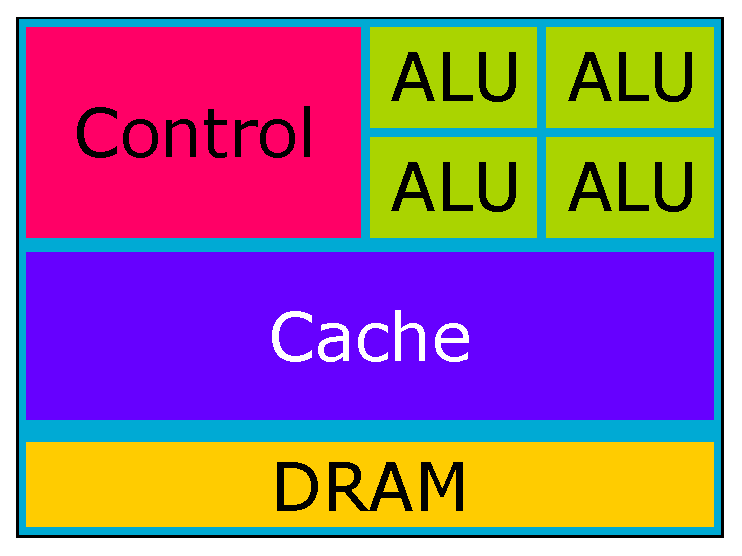
\includegraphics[width=1\linewidth]{img/CPUarchitecture.eps}
  \caption{architektura CPU}
  \label{fig:cpuarchitecture}
\end{subfigure}
\begin{subfigure}{.49\textwidth}
  \centering
  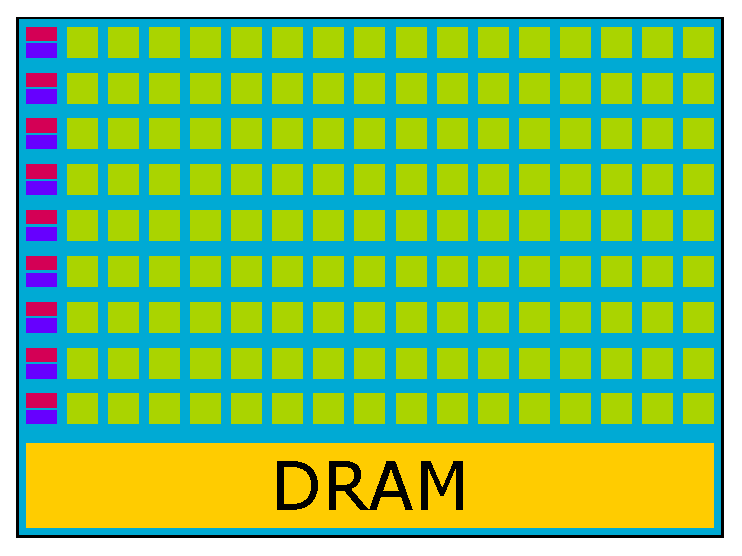
\includegraphics[width=1\linewidth]{img/GPUarchitecture.eps}
  \caption{architektura GPU}
  \label{fig:gpuarchitecture}
\end{subfigure}
\caption{Porovnání architektury CPU a GPU (stejné barvy obdélníku znamenají stejné jendotky)}
\end{figure}

%\begin{table}
%\begin{tabular}{|l|l|l|}
%\cline{1-2}
%NIC & CPU & GPU \\ \cline{1-2}
%# cores & Few cores per chip & Many cores per chip \\ \cline{1-2}
%Specialization & General purpose cores & Cores psecialized for numeric computations \\ \cline{1-2}
%Threads approach & Processing different threads & SIMT thread processing \\ \cline{1-2}
%Memory access & Huge caches to reduce memory latency & Huge amount of threads and fast context switch \\ \cline{1-2}
%\end{tabular}
%\end{table}
\section{CUDA}
CUDA (Compute Unified Device Architecture) je platforma pro paralelní výpočty pro GPGPU vyvíjená společností Nvidia. Zahrnuje jak hardwarovou tak softwarovou architekturu integrovanou na grafických kartách Nvidia. CUDA podporuje více programovacích jazyků, konkrétně C, C++ a Fortran, což ji dělá přístupnější pro vývojáře. Existují i jiné platformy, jako například OpenCL, ale z důvodů popsaných výše se jimi nebudeme zabývat.\\

\begin{figure}[h]
\centering
%\begin{subfigure}{0.49\textwidth}
%  \centering
%  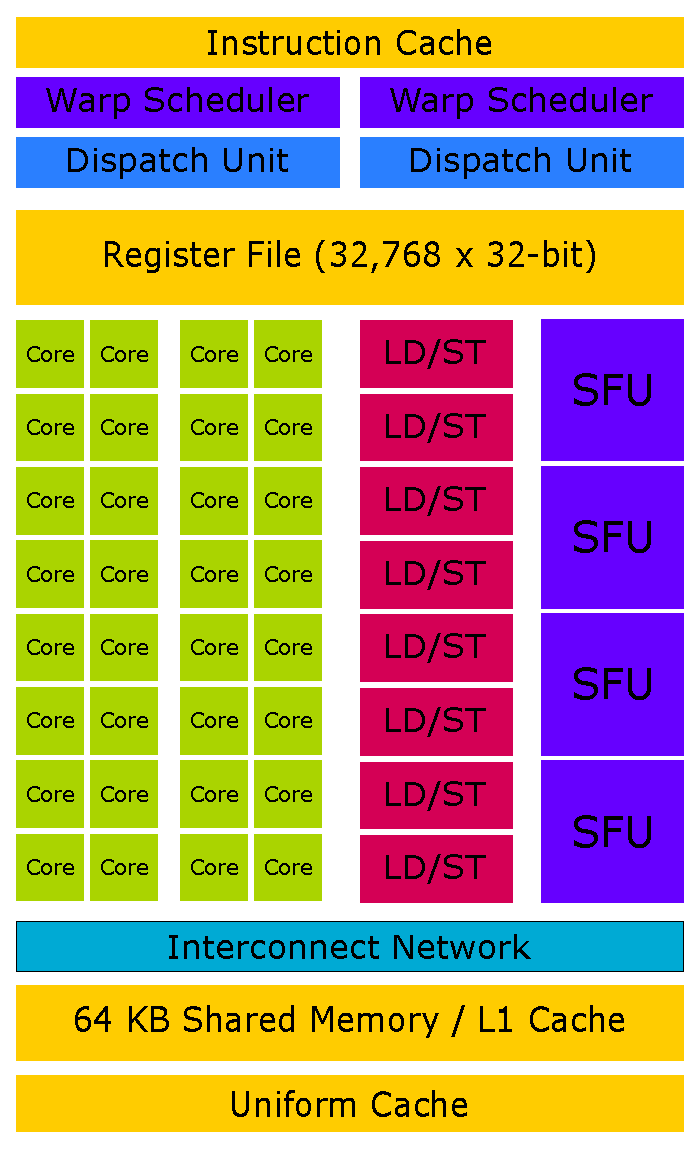
\includegraphics[width=0.8\linewidth]{img/SMPArchitecture.eps}
%  \caption{SMP architecture (Fermi)}
%  \label{fig:smparchitecture}
%\end{subfigure}
%\begin{subfigure}{0.6\textwidth}
  %\centering
  %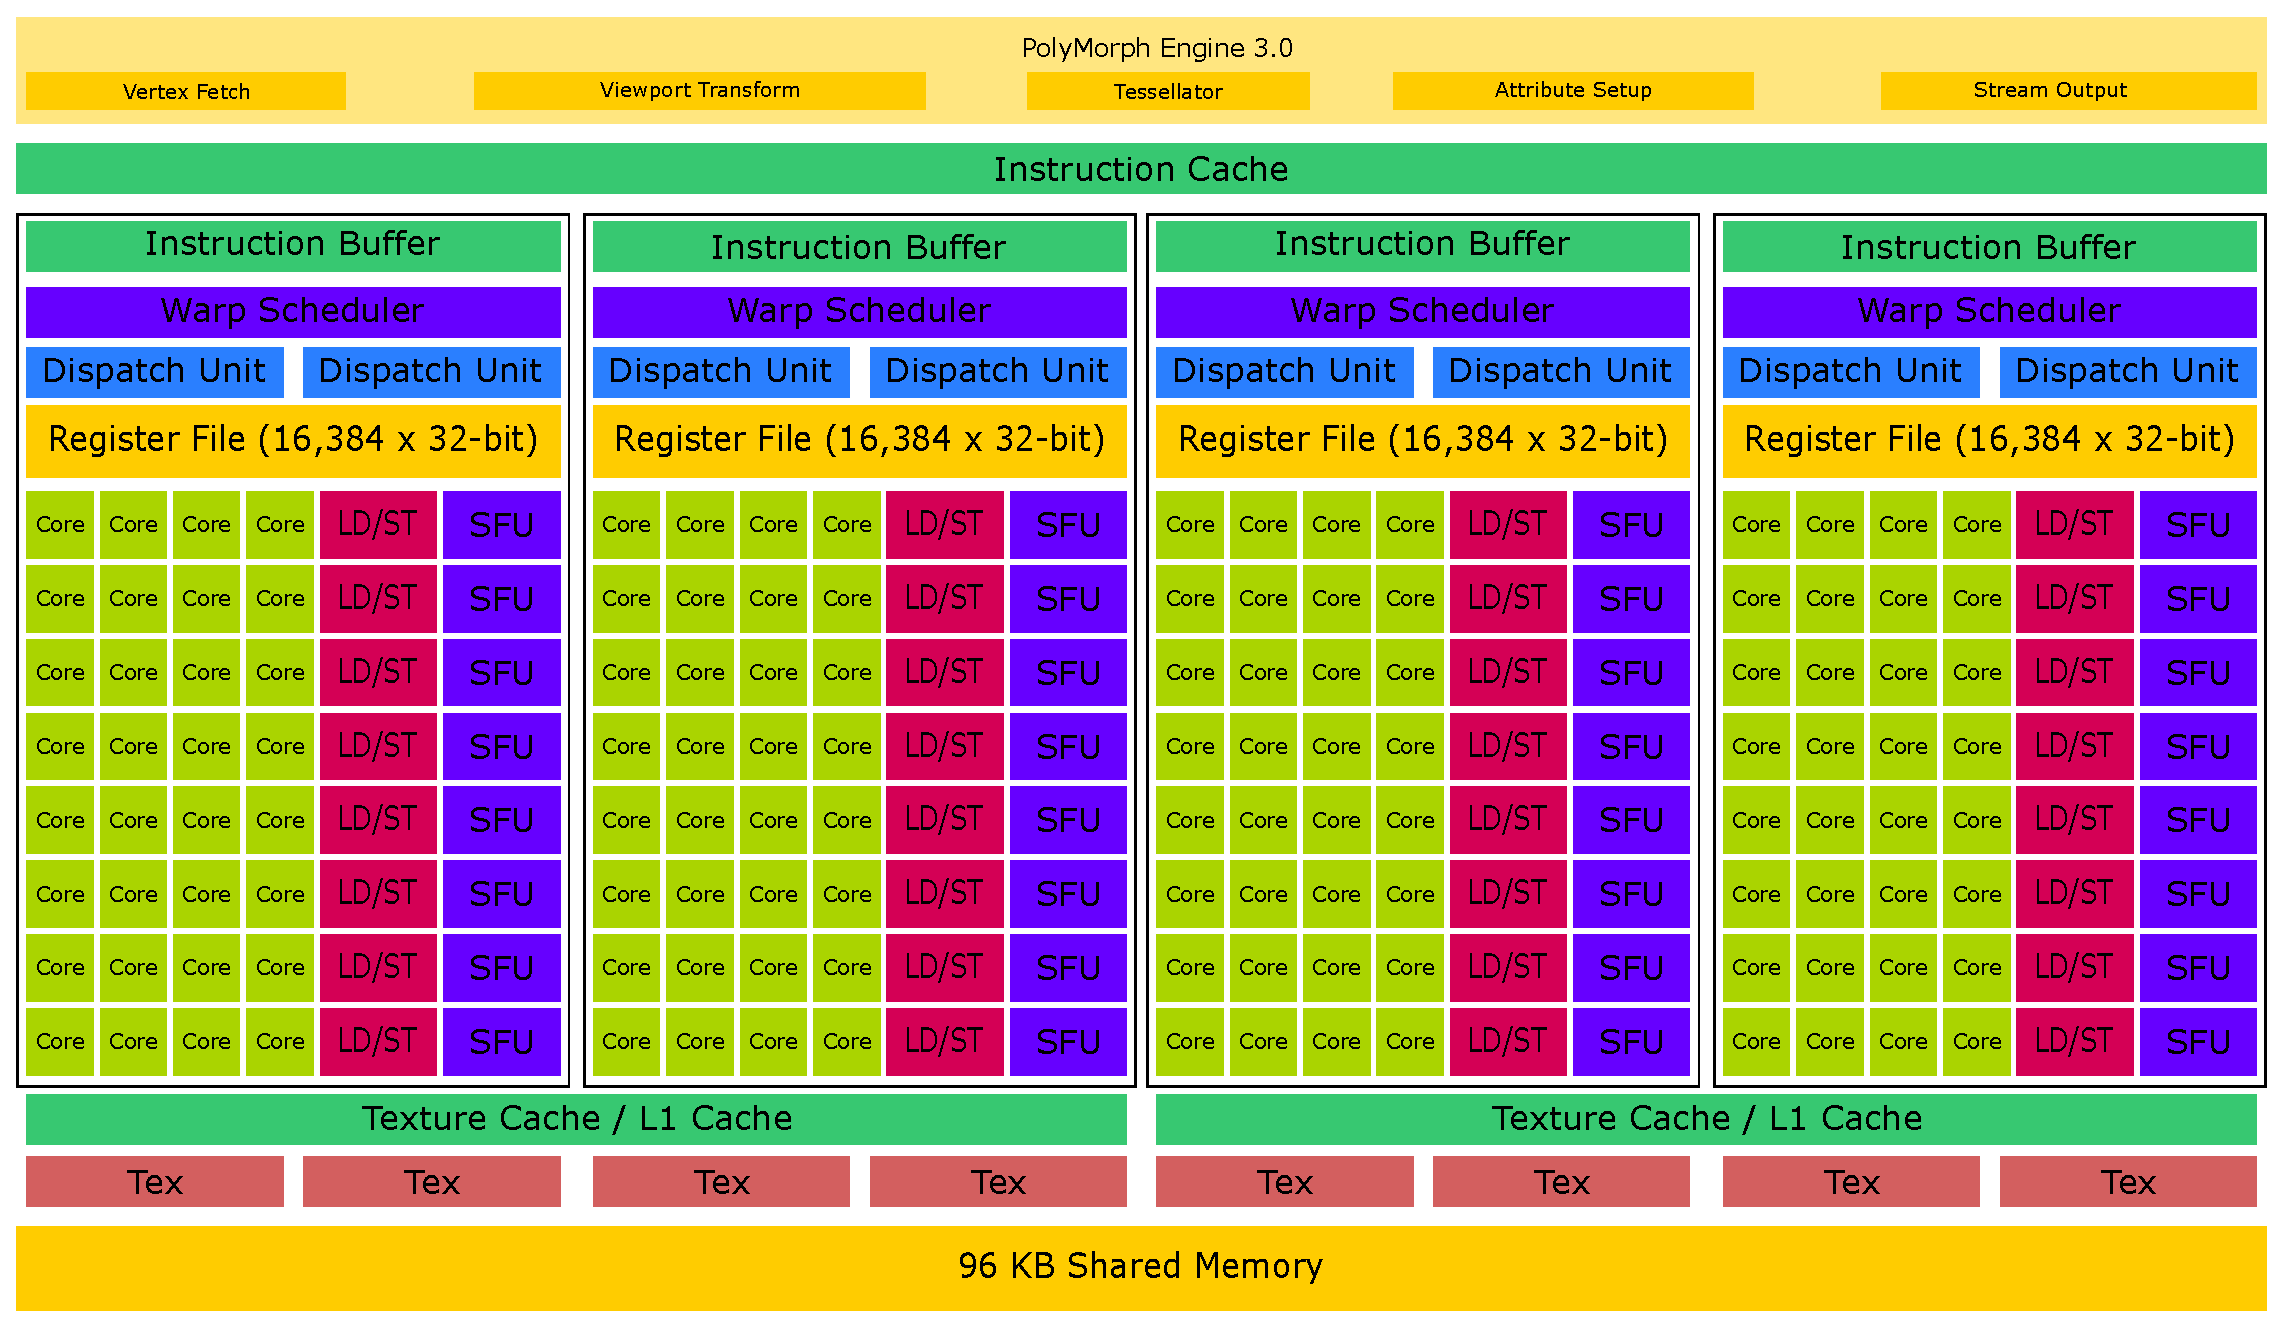
\includegraphics[width=1\linewidth]{img/SMMArchitecture.eps}
  %\caption{Architektura SMM (Maxwell)}
 % \label{fig:smmarchitecture}
  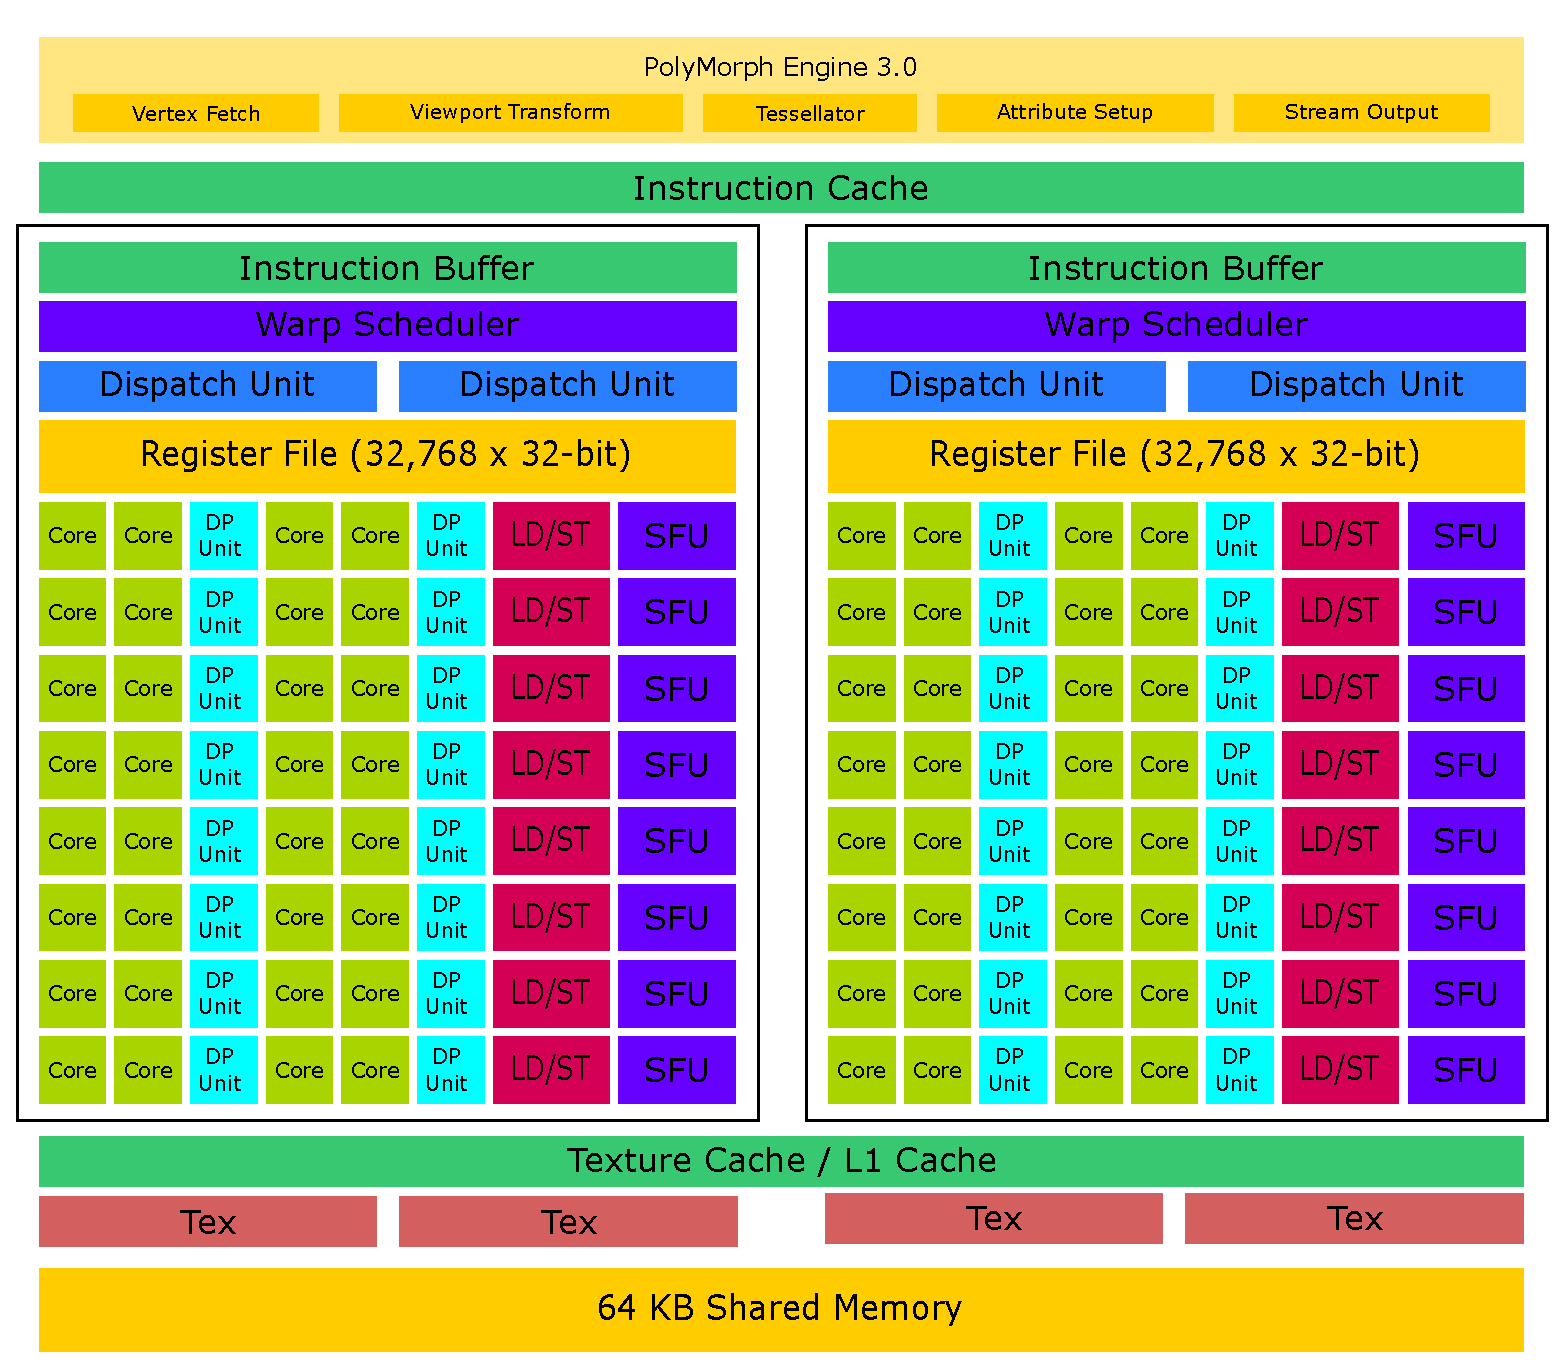
\includegraphics[width=1.0\linewidth]{img/PSMArchitecture.eps}
  \caption{Architektura PSM (Pascal)}
  \label{fig:psmarchitecture}
%\end{subfigure}
%\vspace*{0.1cm} 
%\begin{subfigure}{0.6\textwidth}
%  \centering
%  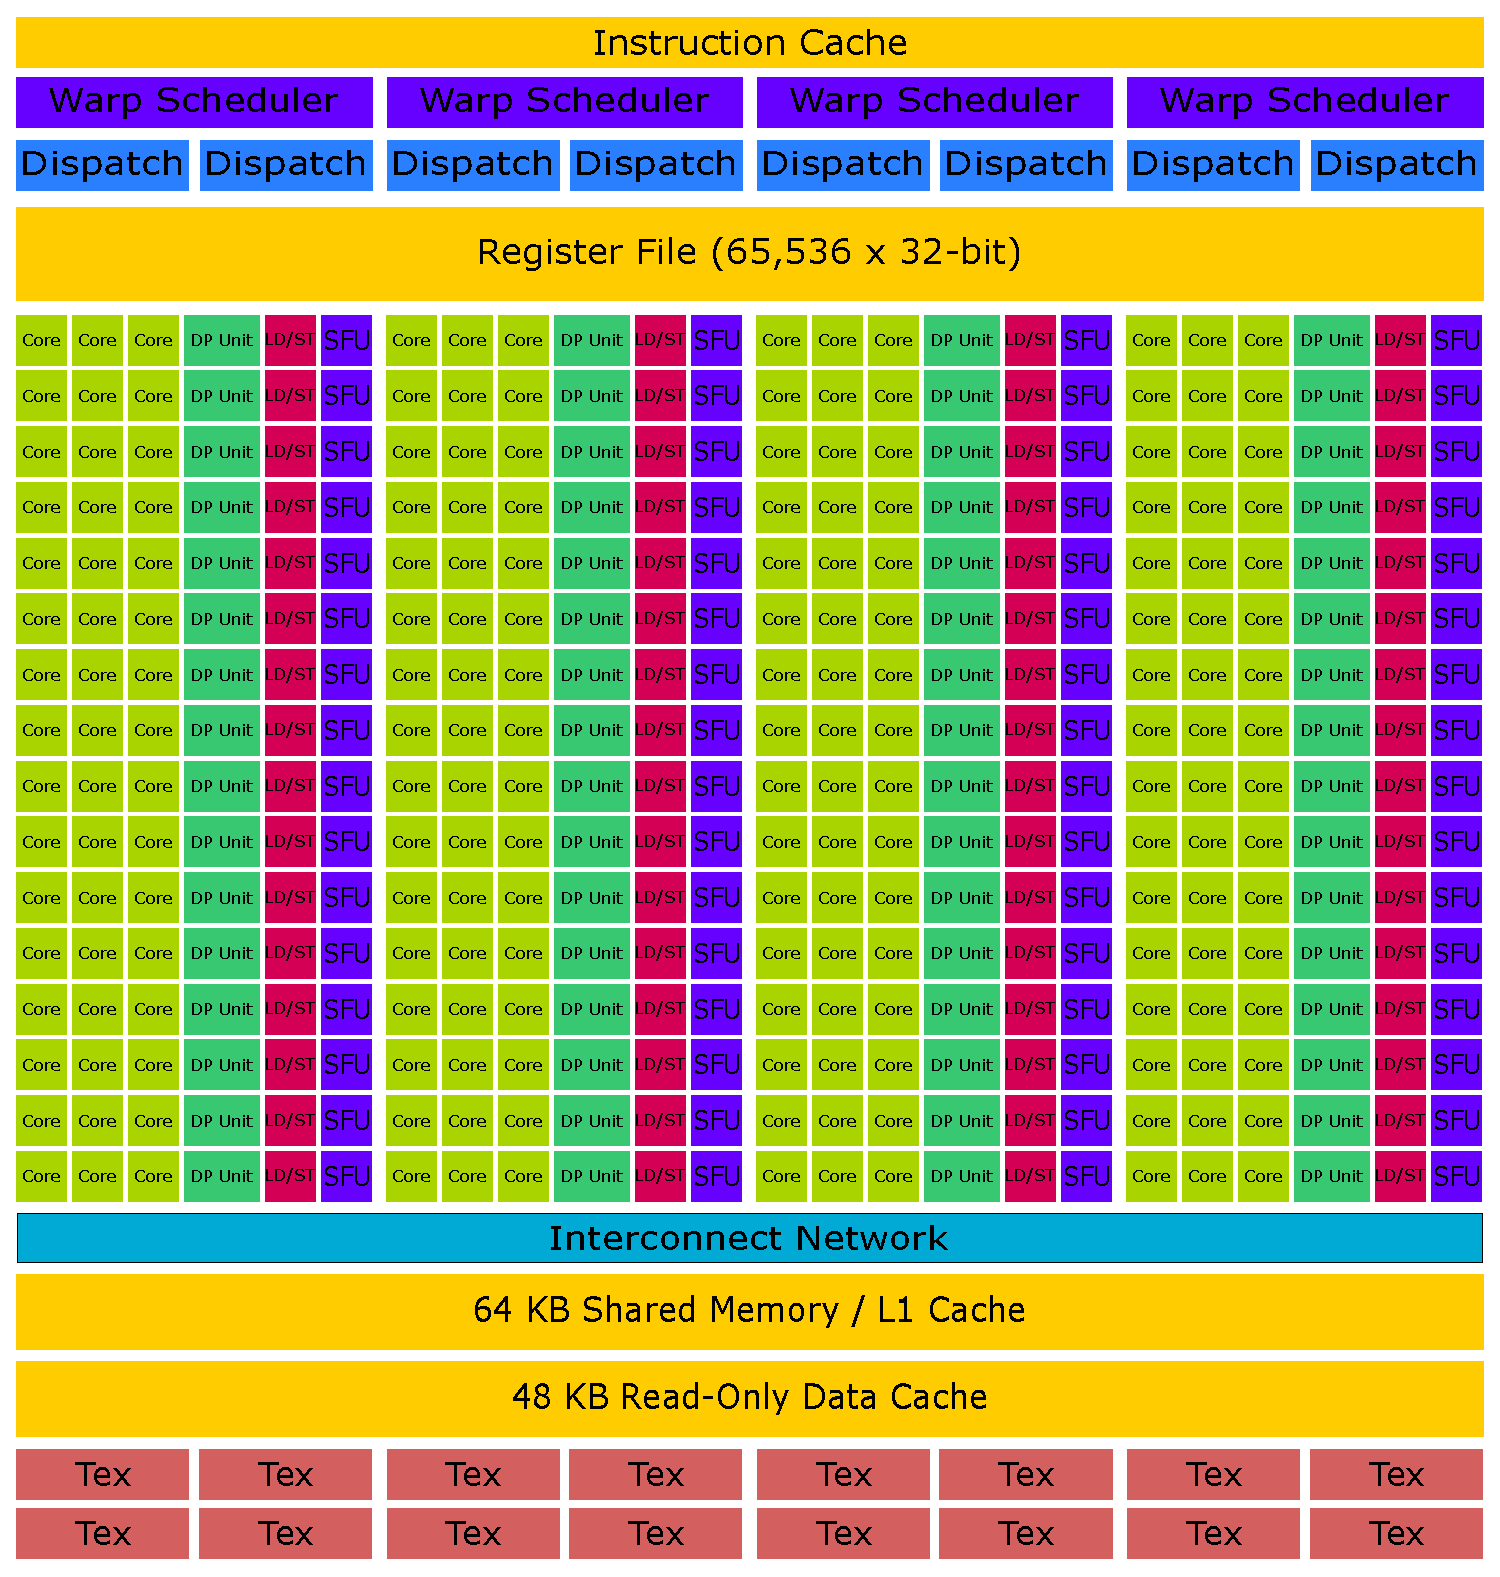
\includegraphics[width=0.9\linewidth]{img/SMXArchitecture.eps}
%  \caption{SMX architecture (Kepler)}
%  \label{fig:smxarchitecture}
%\end{subfigure}
\end{figure}

CUDA architektura obsahuje více větších procesorů zvaných \textbf{Streaming Multiprocessor (SMP)}. Nejstarší generací je \textbf{SM} - Fermi, následuje \textbf{SMX} - Kepler, novější \textbf{SMM} - Maxwell a nejnovější \textbf{PSM} - Pascal~(\autoref{fig:psmarchitecture}). Každý SMP obsahuje výpočetní jádra s registry (32 na architektuře Fermi, 64 na architektuře Pascal, 128 na architektuře Maxwell a 192 na architektuře Kepler), načitací a zápisové jednotky (load/store - LD/ST), jednotky pro speciální funkce (SFU), sdílenou instrukční cache, sdílenou paměť (shared memory) a datovou cache (data cache). LD/ST a SFU jednotky jsou sdíleny skupinami jader. Velikost těchto skupin závisí na konkrétní architektuře. Architektura Pascal navíc obsahuje ke každým 2 jednotkám pro single floating point operace ještě jednu double floating ponint jednotku (DP).\\

\begin{figure}[h]
  \centering
  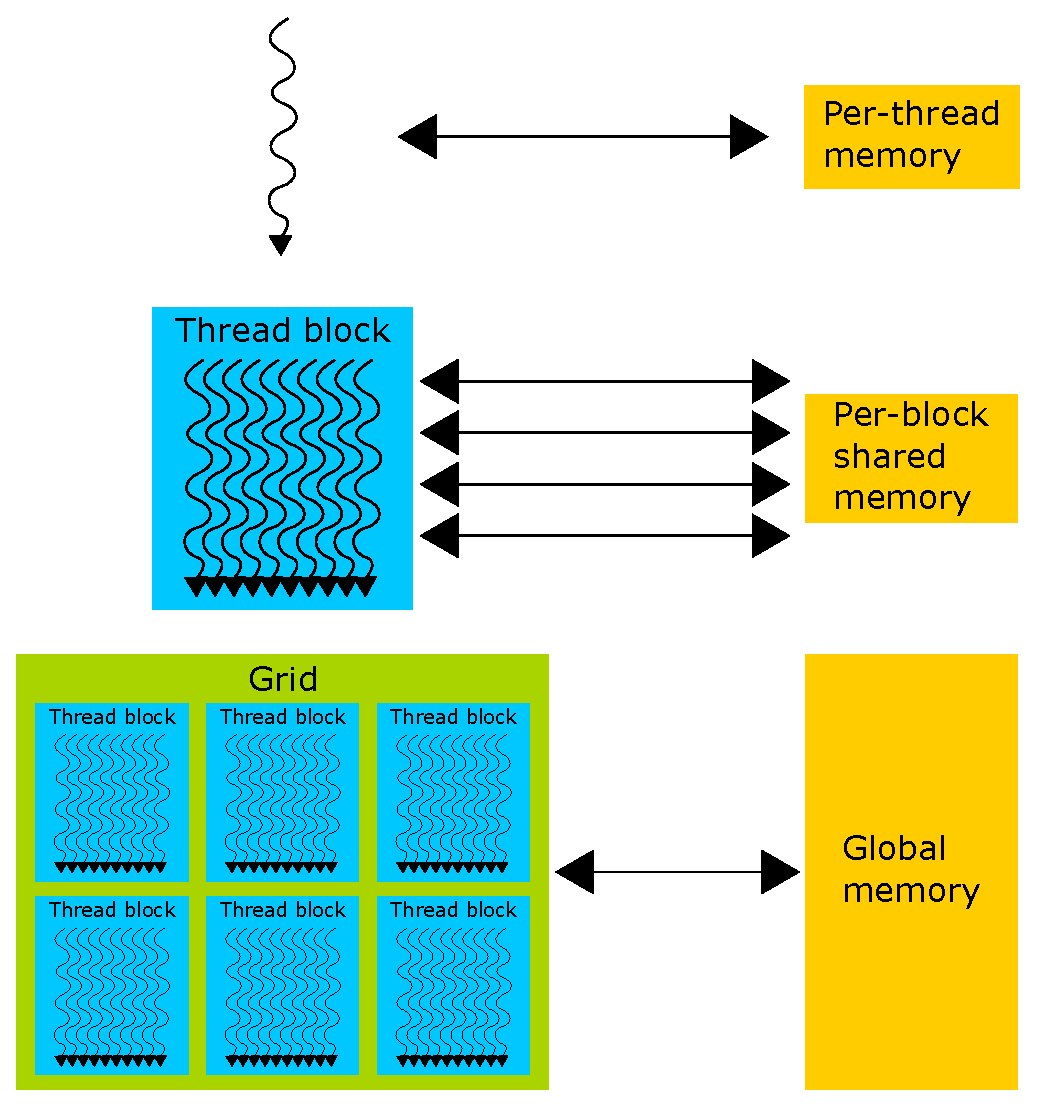
\includegraphics[width=0.8\linewidth]{img/CUDAmemoryHierarchy.eps}
  \caption{Výpočetní model CUDA}
  \label{fig:cudamemhierarchy}
\end{figure}

Dalším parametrem odlišující jednotlivé CUDA zařízení je \textbf{Compute Capability} (CC), která udává vlastnosti zařízení a sadu instrukcí, které jsou podporované. CC je úzce spjatá s architekturou(CC 1.x byla podporována architekturou Tesla, CC 2.x na Fermi, 3.x na Kepleru, 5.x na Maxwellu a 6.x na Pascalu).\\

CUDA využívá modelu Simple Instruction Multiple Thread (SIMT). Tento model přistupuje k paralelizaci tak, že je jedna instrukce vykonávána více výpočetními jednotkami, takže stačí pouze jedna fetch/decode jednotka pro načítání instrukcí pro celou skupinu výpočetních jednotek. Tento model je podobný modelu Simple Instruction Multiple Data (SIMD), ale rozdíl je v tom, že SIMT má více registrů. SIMD jednoduše zpracovává malé vektory paralelně a všechna vlákna dělají tu samou operaci. Pokud tedy chceme například sešíst 2 vektory, SIMD musí iterovat přes celý vektor a v každém kroku může zpracovat tolik prvků, kolik má výpočetních jednotek.Oproti tomu CUDA se SIMT modelem může nastartovat tolik vláken, jako je velikost vektoru a každé vlákno si pak výsledek uloží ve svém registru.\\

\subsection{Běh CUDA programu}
Pokud chceme spustit program CUDA, první, co musíme udělat, je detekovat v systému CUDA zařízení. Po jeho zvolení můžeme začít kopírovat data ze hostujícího systému na CUDA zařízení. tato operace je asynchronní, takže ji musíme synchronizovat s výpočtem na kartě. Jakmile jsou data zkopírována, můžeme začít s vykonáváním výpočtu pomocí volání speciálních metod zvaných \textbf{kernel} (jádro). Jádro se chová stejně jako běžná funkce v C, ale běží přímo na GPU a má tedy přístup ke speciálním funkcím specifikovaných v CC.\\ 

Dalším rozdílem je jeho volání. Jádro totiž běží asynchronně a navíc musíme, kromě vlastních parametrů, přidat i parametry pro paralelizaci. Jedním parametrem určíme, kolik vláken má jedna instance jádra k dispozici. Vlákna jsou navíc organizovány v jedno-, dvou- nebo tří-rozměrném prostoru a tak, pokud je to vhodné, můžeme jednoduše reflektovat vlastnosti vstupních dat, nad kterými výpočet běží. Tomuto balíku vláken se říká \textbf{blok}. Počet vláken v jednom bloku je omezen, protože všechna musí běžet na jediném multiprocesoru a musí sdílet jeho omezenou paměť. Na současných GPU je tedy maximální počet vláken 1024.\\

Dalším parametrem volání je počet bloků, který udává, v kolika instancích se má jádro spustit. Bloky jsou, stejně jako vlákna, organizovány ve jedno-, dvou- nebo tří-rozměrném prostoru. Tato struktura se nazývá \textbf{grid}. Jediným omezením gridu je, že musí být všechny stejně velké a tak se většinou jejich počet volí podle velikosti dat nebo podle počtu multiprocesorů. Celkový počet vláken vykonávaných jedním jádrem tak je počet vláken vynásobený zvoleným počtem bloků~(\autoref{fig:cudagridthreadblock}).\\

Jelikož je vlákno voláno asynchronně, může host po dobu jeho vykonávání pracovat na jiných úlohách, jako například kopírování dat pro další výpočet. Po doběhnutí jádra obvykle potřebujeme přesunmout výsledky zpět na hostitelský stroj, což je opět asynchronní operace,\\

\begin{figure}[h]
  \centering
  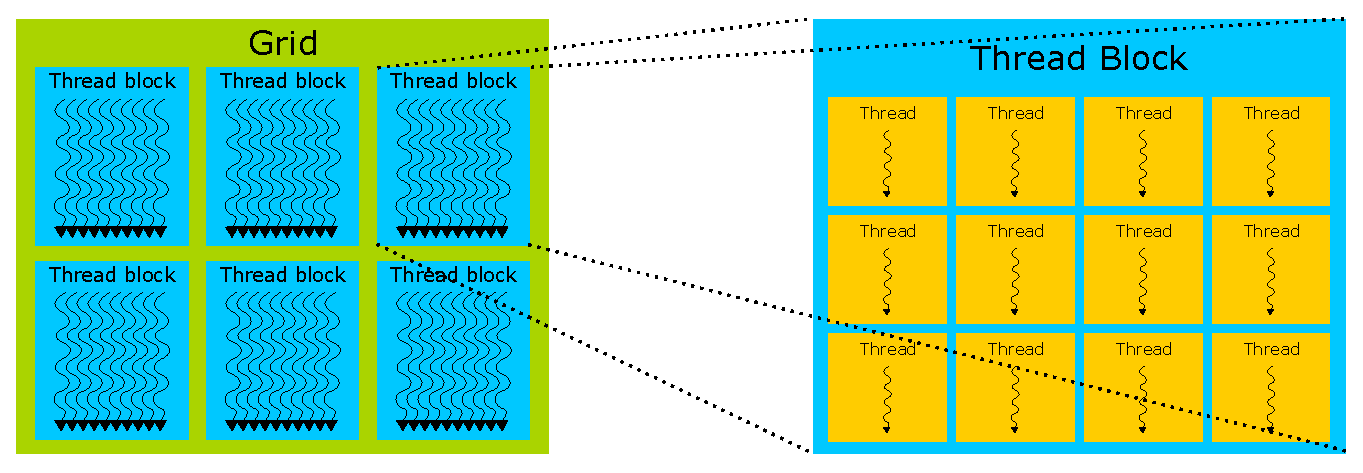
\includegraphics[width=1\linewidth]{img/CUDAthreadGridBlock.eps}
  \caption{dvou-dimenzionální grid dvou-dimenzionálních bloků vláken}
  \label{fig:cudagridthreadblock}
\end{figure}

Protože počet fyzických jader je většinou menší než počet vláken, se kterými je spuštěn kernel, mohou současně běžet jen některá vlákna. Takovým blokům se říká \textbf{warp}. Když spustíme kernel, každá blok je přiřazen jednomu multiprocesoru a v průběhu již nemigruje jinam. Každý SMP pak bloky rozdělí do warpů v závislosti na konkrétní architektuře (počtu fyzických jader na SMP). Rozdělení práce do bloků a vláken může mít velký vliv na efektivitu algoritmu. Pokud zvolíme špatnou velikost bloku, nedělitelnou velikostí warpu, nevyužijí některé z warpů všechna jádra jednoho SMP. Spustíme-li tedy kernel v 8 blocích, každý po 96 vláknech, bude blok rozdělen na 3 warpy a celkem tedy poběží 24 warpů. Pokud bychom ale kernel spustili s 64 bloky o 12 vláknech, každá warp by využil pouze 12 vláken a celkově bychom SMP musel spustit 64 warpů a výpočet by tedy trval skoro třikrát déle. Je to dáno tím, že CUDA neumí spojit vlákna z různých bloků do jednoho warpu. Proto se doporučuje zvolit velikost bloku tak, aby byl dělitelný velikostí warpu.\\

CUDA omezuje také typy operací, které mohou být vykonávány v jeden okamžik. Například na architektuře Kepler mohou vykonávat pouze 4 z 12 skupin jader operace s desetinou čárkou s dvojitou přesností (double floating point). takže u tohoto typu operace může dojít až trojnásobnému zpomalení. Jelikož ale může ostatních 8 skupin vláken dělat jiné operace (například celočíselné), zpomalení je většinou menší.\\

Problematická je ale práce s pamětí. Běžné CPU používá k zakrytí latence víceúrovňovou paměť cache. Ta je k dispozici i na architektuře CUDA~(\autoref{fig:cudamemhierarchy}), ale protože je CUDA uzpůsobena především k proudovým výpočtům s vysokou propustností, je cachování paměti neefektivní. Tento problém je na CUDA běžně řešen tak, že na jendom SMP existuje více aktivních warpů a v momentě, kdy jeden z warpů potřebuje vykonat paměťovou operaci, SMP spustí jiný připravený warp. Tento mechanismus udržuje výpočetní jádra vytížená jak je možné, čímž je výpočet efektivnější.\\
 
Vlákna v jednom bloku tedy sdílí paměťové cache a běží na jednom SMP. Navíc mohou být vlákna v jednom warpu synchronizována. Naproti tomu vlákna z různých warpů mohou být přiřazena jinému SMP a nebo mohou být vykonávána současně na stejnému SMP.\\

\subsection{Paměťový model}

Paměťový model na architektuře CUDA~\ref{fig:cudamemaccess} se skládá z více typů pamětí, které se liší především svou velikostí, propustností a latencí.

\begin{figure}[h]
  \centering
  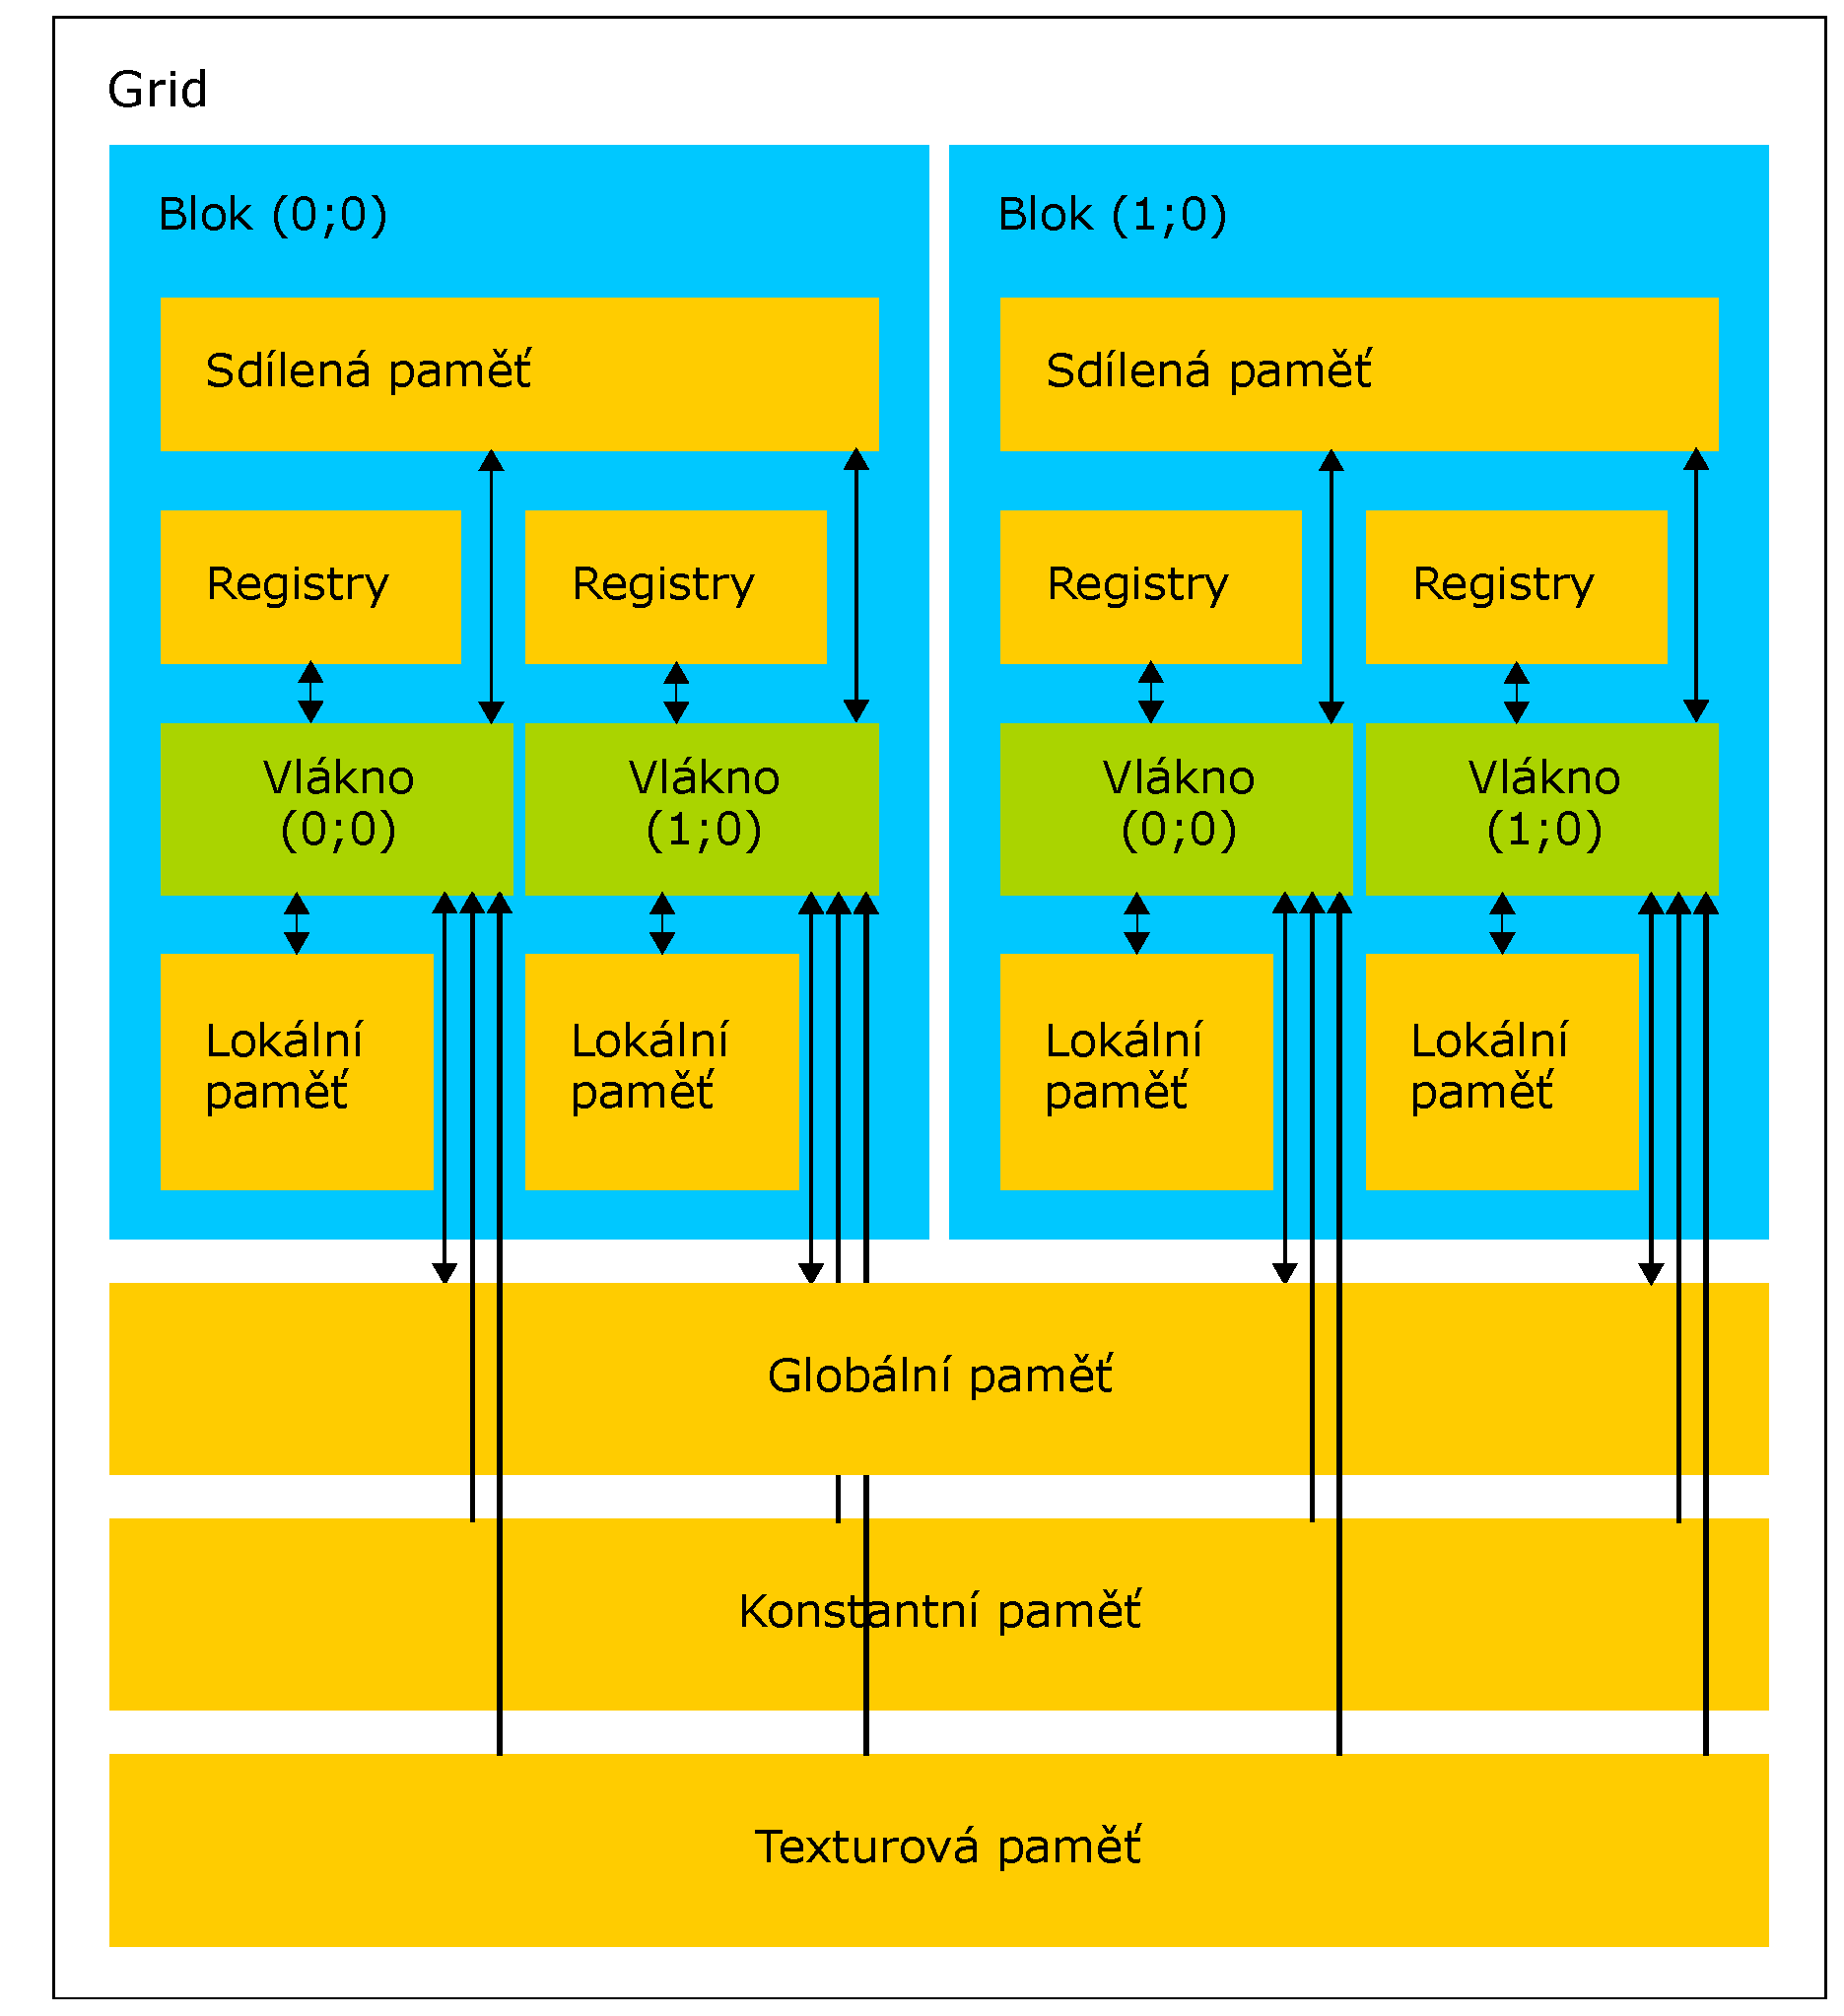
\includegraphics[width=0.6\linewidth]{img/CUDAmemAccess.eps}
  \caption{Přístu ke CUDA pamětím}
  \label{fig:cudamemaccess}
\end{figure}

\begin{description}
\item[Globální paměť] je pamět s kapacitou v řádech gigabajtů a je tak největší pamětí na GPU. Má také velice vysokou propustnost (kolem 100 GB/s), ale má vysokou odezvu (400 až 600 taktů). Pro výpočet může být alokována jako CUDA pole, což je paměť optimalizovaná pro cachování textur, nebo jako lineární paměť. Ta leží celá v 40bitovém adresovém prostoru a tak se na ni můžeme  odkazovat pomocí ukazatelů.~\cite{CUDAGuide} Slouží především k ukládání dat přesunutých z hosta. Spravuje se (alokace a uvolňování) z hostitelského kódu pomocí speciálních CUDA API funkcí před během programu na GPU. Alokace globální paměti je nezávislá na běhu jednotlivých kernelů (s výjimkou dynamicky alokované paměti při běhu kernelu). Díky tomu může být využita více kernely aniž by musela být po každém běhu dealokována a znovu alokována. Při práci z globální pamětí jsou také velice důležité funkce pro přesun dat z hosta na CUDA zařízení a zpět. Jde opět o speciální funkce z CUDA API, které jsou volány asynchronně. Stejně jako u alokace/dealokace jsou i data zachována mezi běhy jednotlivých kernelů. Při přístupu k datům v globální paměti dochází ke cachování v L2 cache paměti. Tato paměť je také vyuýívána pře přesunu dat mezi hostem a GPU. Pracuje v transakcích o velikosti 32 bajtů až 128 bajtů, takže pro lepší výkonnost je dobré data zarovnat s velikostí transakce. Fyzicky se nachází mimo GPU čip, ale dostatečně blízko na kartě, aby byl k ní bylo možné rychle přistupovat. 

\item[Sdílená paměť] je paměť dostupná ze všech vláken běžících na stejném SM. Má menší odezvu než globální paměť (32 bitů za 2 takty na CC 1.x a 2.x a 64 bitů za jeden takt na CC 3.x a novějších), ale je také oproti globální paměti menší (opět v závislosti na CC od 16 kB na 1.x po 48 kB na novějších). Může být stejně rychlá jako registry, pokud nedojde k tzv. bankovním konfliktům (viz další odstavec). Sdílená paměť má závislé čtení na zápisu. To znamená, že trvá 24 taktů, než je možné zapsaná data přečíst. Tato omezení jde ale obejít dostatkem aktivních warpů, které mohou mezitím běžet. Ve sdílené paměti se uchovávají staticky alokované proměnné a také dynamický blok paměti alokovaný při startu kernelu. K uvolnění paměti dochází automaticky po skončení běhu kernelu, takže data zde uložená nejsou mezi zachována ani mezi jednotlivými běhy stejného kernelu. \\

Tato paměť je rozdělená do bank, což jsou bloky paměti, ke kterým je možné přistupovat nezávisle. Tím se stává sdílená paměť velice rychlou, ale musíme dávat pozor na bankovní konflikty. Ty nastanou, pokud do jedné banky přistupuje více vláken naráz a přístup probíhá sériově (až na případ, kdy čteme ze stejné adresy, kdy dojde k rozeslaní daných dat, tzv. broadcastu). Při takovém konfliktu dochází k výraznému zpomalení běhu a je tedy dobré se bankovním konfliktům vyhnout. Toho lze docílit tak, že jednotlivá vlákna přistupují k bankám lineárně~(\ref{fig:linearaccess}) nebo s daným posunem~(\ref{fig:strideaccess}), který není soudělný s počtem bank. Na starších CC (1.x a 2.x) je velikost banky 32 bitů, od CC 3.0 si můžeme vybrat mezi 32 a 64 bitovými bankami. Fyzicky je sdílená paměť umístěna velmi blízko procesoru kvůli rychlému přístupu. 
\end{description}

\begin{figure}[h]
\centering
\begin{subfigure}{1.0\textwidth}
  \centering
  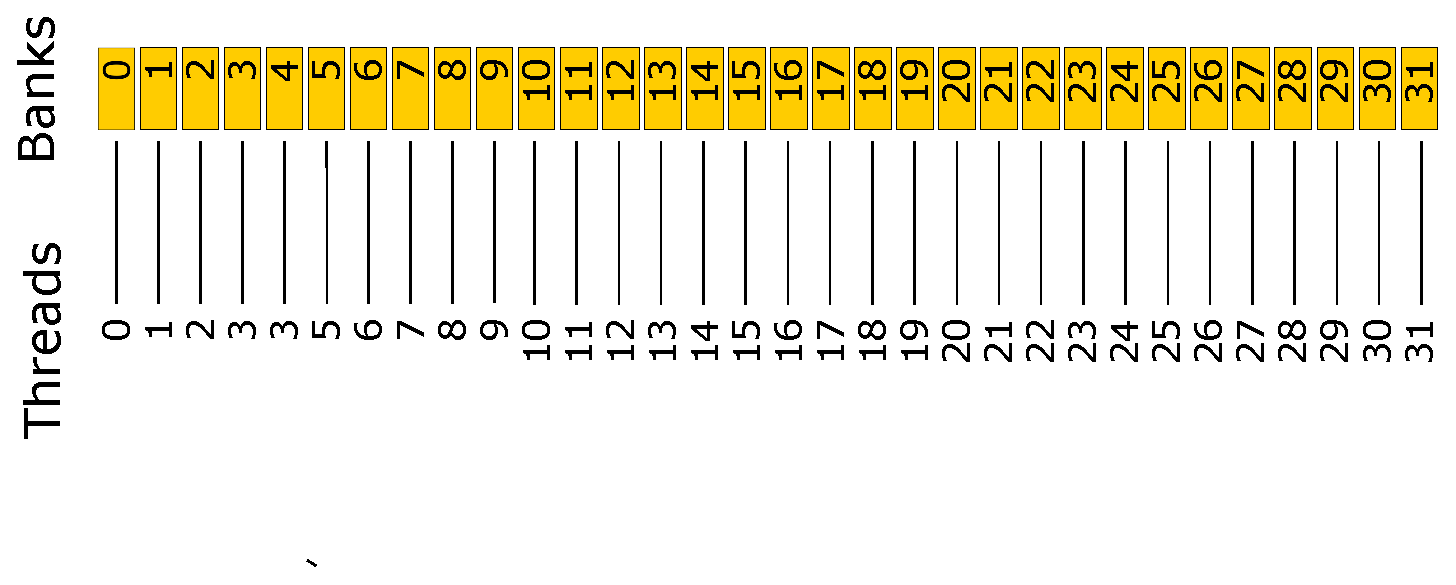
\includegraphics[width=.9\linewidth]{img/sharedMemoryLinearAccess.eps}
  \caption{Lineární přístup ke sdílené paměti}
  \label{fig:linearaccess}
\end{subfigure}
\begin{subfigure}{1.0\textwidth}
  \centering
  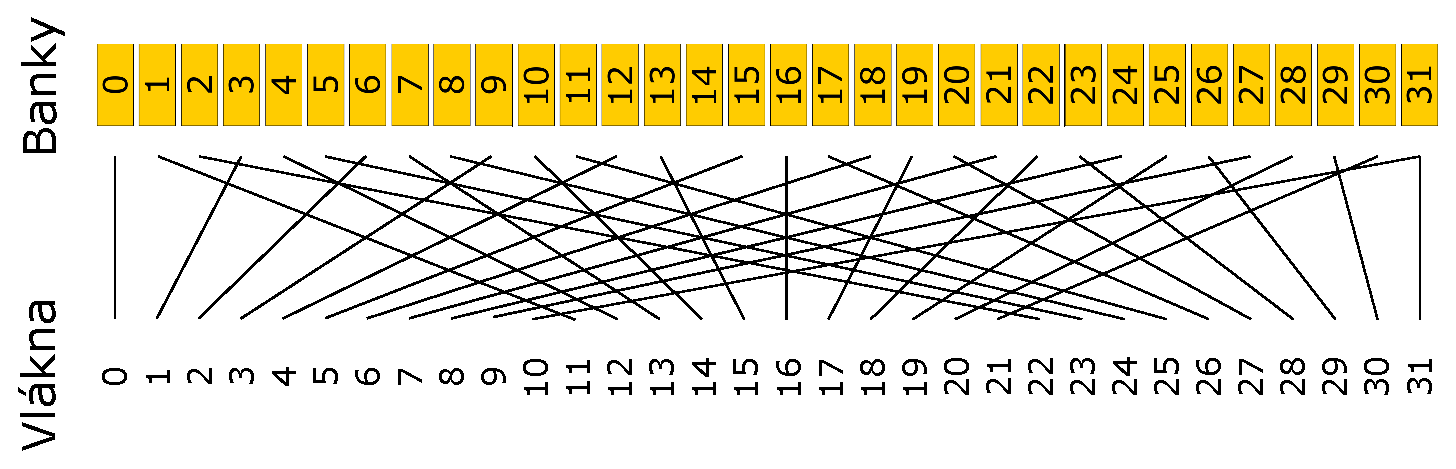
\includegraphics[width=.9\linewidth]{img/sharedMemoryStrideAccess.eps}
  \caption{Přístup ke sdílené paměti s posunem}
  \label{fig:strideaccess}
\end{subfigure}
\caption{Přístup ke sdílené paměti}
\end{figure}

\begin{description}
\item[L1 Cache] má na většině zařízení stejné parametry jako sdílená paměť, protože využívá stejného hardware. Cachujá se v ní přístupy do lokální a globální paměti, takže výrazně urychluje přístup k datům (100x až 150x). Díky speciálnímu CUDA API je možné před výpočtem nakonfigurovat, která paměť bude upřednostněna. Od CC 5.x je L1 cache sloučena s texturovou pamětí a je nezávislá na sdílené paměti (nesdílí stejné prostředky).

\item[Registry] Každý multiprocesor má vlastní sadu registrů. V závislosti na CC je to buď 8 až 64 kilobajtů 32-bitových registrů. Registry jsou nejmenší paměť, ale mají také nejmenší latenci (jsou stejně rychlé jako procesor). Registry nejsou programátorsky přístupné přímo. Jediné zpoždění je, podobně jako u sdílené paměti, závislost čtení na zápisu, které trvá 24 cyklů, ale může být také podobně skryto pomocí dostatku aktivních warpů. Pokud používá jádro více registrů, než je dostupná velikost, jsou registry uloženy v lokální paměti. Tonto problém se nazývá \textit{registry spilling}.\\

Každé vlákno má svoji sadu registrů. Počet a velikost registrů na vlákno a velikost bloku určuje, kolik bloků může být alokováno na jednom multiprocesoru. Například na CC 2.x, pokud kernel používá 32 registrů a každý blok obsahuje 512 vláken, tak na jednom multiprocesoru můžou být 2 bloky, které vyžadují $2\times512\times32$ registrů, což přesně odpovídá počtu registrů dostupných na multiprocesoru. Jakmile by kernel používal jen o jeden registr navíc, může být na multiprocesoru pouze jeden blok~\cite{CUDAGuide}.

\item[Lokální paměť] je paměť vyhrazená v globální paměti a je přístupná pouze jedním vláknem. V lokální paměti jsou uloženy pouze některé automatické proměnné~\cite{CUDAGuide}:
\begin{itemize}
\item Pole, u kterých není možní zjistit, zda jsou indexovaná konstantními hodnotami
\item Velké struktury polí, které by spotřebovali příliš mnoho registrů
\item Jakákoliv proměnná, pokud kernel využívá více registrů, než je fyzicky dostupných (již zmíněný register spilling).
\end{itemize}
Přístup do lokální paměti je na CC 2.x a starších vždy cachován v L1 a L2 paměti. Na novějších CC je přístup do lokální paměti vždy cachován pouze v L2 cache.
\item[Konstantní paměť] je speciální paměť určená pouze pro konstantní data. Její velikost je 64kB a od CC 2.x zde kompilátor uchovává konstantní proměnné nezávislé na vláknech. 
\item[Paměť pro textury] je speciální typ paměti určený pro grafiku. Její výhodou je 2D prostorová lokalita využívaná především texturami.
\end{description}

Přenos dat mezi hostem a GPU je mnohem pomalejší než přesuny mezi paměťmi samotné GPU. Úzkým hrdlem je sběrnice PCI Express, která má v závislosti na verzi propustnost 16-32 GB za sekundu a navíc může bát ještě zpomalena hostem v případě, kdy jsou některá kopírovaná data uložena na pevném disku. Samotný přesun dat má také nezanedbatelnou režii, což může vést k neefektivnímu výpočtu na CUDA zařízení v případě, že potřebujeme počítat malé úlohy a přesouvat malá data. Tato nevýhoda se řeší pomocí hromadného přesunu velkého objemu dat namísto kopírování jednotlivých bloků paměti. Další možností je využít asynchronosti kopírování a samotného výpočtu, protože CUDA zařízení je schopné v jeden okamžik provádět až dva nezávislé přesuny data a zároveň vykonávat výpočet, takže můžeme kopírovat data pro budoucí iteraci výpočtu na GPU, zároveň provádět výpočet na aktuálními daty a ještě kopírovat výsledky z předchozí iterace zpět do paměti hosta.\\

Paměť na straně hosta může být \textit{připnutá} (pinned), což může urychlit přesun dat na systémech s FSB (Front side bus). Připnutá paměť může být také využita k \textit{namapované paměti} (Mapped memory), která umožní eliminovat přenos dat mezi hostem a GPU díky namapování obou pamětí do stejného adresového prostoru. Všechny přesuny dat jsou pak prováděny implicitně v momentě, kdy jsou vyžádány z běžícího kernelu.